\documentclass[12pt,a4paper]{article}
\usepackage{indentfirst}
\usepackage{fontspec}
\usepackage{graphicx}
\usepackage{float}
\usepackage{subfigure}
\usepackage{wrapfig}
\setmainfont{Times New Roman}
\usepackage{hyperref}
\hypersetup{
    colorlinks=true,
    linkcolor=blue,
    filecolor=magenta,      
    urlcolor=cyan,
    pdftitle={Overleaf Example},
    pdfpagemode=FullScreen,
    }

\urlstyle{same}
\begin{document}
\begin{titlepage}
   \begin{center}
       \vspace*{1cm}

       \textbf{\Huge{Music Feature}}

       \vspace{0.5cm}
        \Large{Music Genre Classification}
            
       \vspace{1.5cm}

       \textbf{Yi-Hsin Lu}

       \vfill
            
        Final Presentation for Statistical Machine Learning
            
       \vspace{0.8cm}
     
       \includegraphics[width=0.4\textwidth]{NDHU_logo.png}
            
       National Dong Hwa University\\
       June 19, 2022
   \end{center}
\end{titlepage}

\tableofcontents

\newpage

\addcontentsline{toc}{section}{Abstract}
\section*{Abstract}
Music genre can be predicted by using Fourier transform and waveform analysis from audio to numerical data. For the model I used like SVM and Random Forest, the result was better than the others in Kaggle.


\section{Introduction}
\subsection{Motivating Question}
When I was a child, I started learning chinese music instrument. That was the beginning that having fun for the music, and I realized the music is also a part of science. For an example, A440 is the musical pitch corresponding to an audio frequency of 440 Hz (from Wikipedia), and every instruments have their own waveform. So I decided to have my master degree for the researching that I want to use my statistics knowledge on the music I learned before. The music topic is the work direction for statistical machine learning project.

\subsection{Focus Problem}
A dataset in Kaggle interests me, 1000 audio tracks each 30 seconds long, it contains 10 genres, each represented by 100 tracks. So my problem is:\\
1. Is the music genre classified by those numerical data?\\
2. If it can be classified, which model is the best for this dataset?

\subsection{Data}
\begin{figure}[h]
    \centering
    \textbf{Music Feature Dataset}\par\medskip
    \begin{center}
        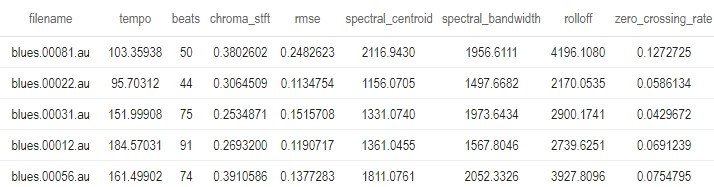
\includegraphics[width=0.8\textwidth]{data_head.jpg}
    \end{center}
\end{figure}

The features in this dataset are extracted from the dataset provided it which consists of 1000 audio tracks each 30 seconds long. It contains 10 genres, each represented by 100 tracks. The tracks are all 22050 Hz Mono 16-bit audio files in .wav format. The code used to extract features is at this GitHub repo. Features are extracted using libROSA library. (Content in kaggle)

\subsection{Variables/Features}
\begin{itemize}
  \item tempo: The speed at which a passage of music is played
  \item beats: Rhythmic unit in music
  \item chroma-stft: Short Time Fourier Transform
  \item rmse: Root Mean Square Error
  \item spectral-centroid: Indicates where the “center of mass” of the spectrum is located.
  \item spectral-bandwidth: It is the Wavelength interval in which a radiated spectral quantity is not less than half its maximum value.
  \item rolloff: Roll-off is the steepness of a transmission function with frequency.
  \item zero-crossing-rate: The rate at which the signal changes from positive to negative or back.
  \item mfcc1-20: Mel-frequency cepstral coefficients (MFCCs) are coefficients that collectively make up an MFC.
\end{itemize}

\subsection{Genres (label)}
\begin{itemize}
  \item blues
  \item classical
  \item country
  \item disco
  \item hiphop
  \item jazz
  \item metal
  \item pop
  \item reggae
  \item rock 
\end{itemize}

\newpage
\section{EDA}
\subsection{Correlation Matrix}
\begin{figure}[h]
    \begin{center}
        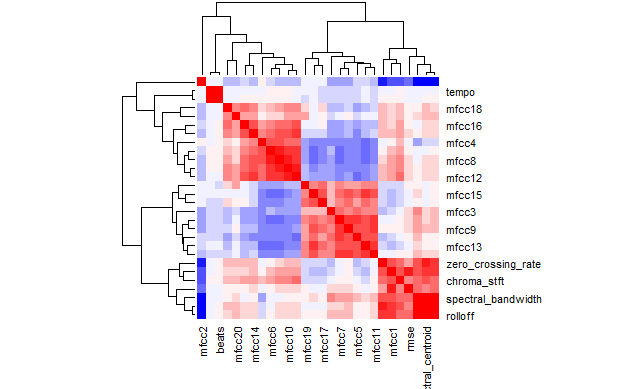
\includegraphics[width=1.2\textwidth]{correlation_matrix.png}
    \end{center}
    \caption{Correlation Matrix}
\end{figure}

It could be splitted by three parts in the red area that is the positive high correlation. Then we made the figure of pairs plot fir these three high correlation area.
\newpage
\subsection{Pairs plot}
\begin{figure}[h]
    \begin{center}
        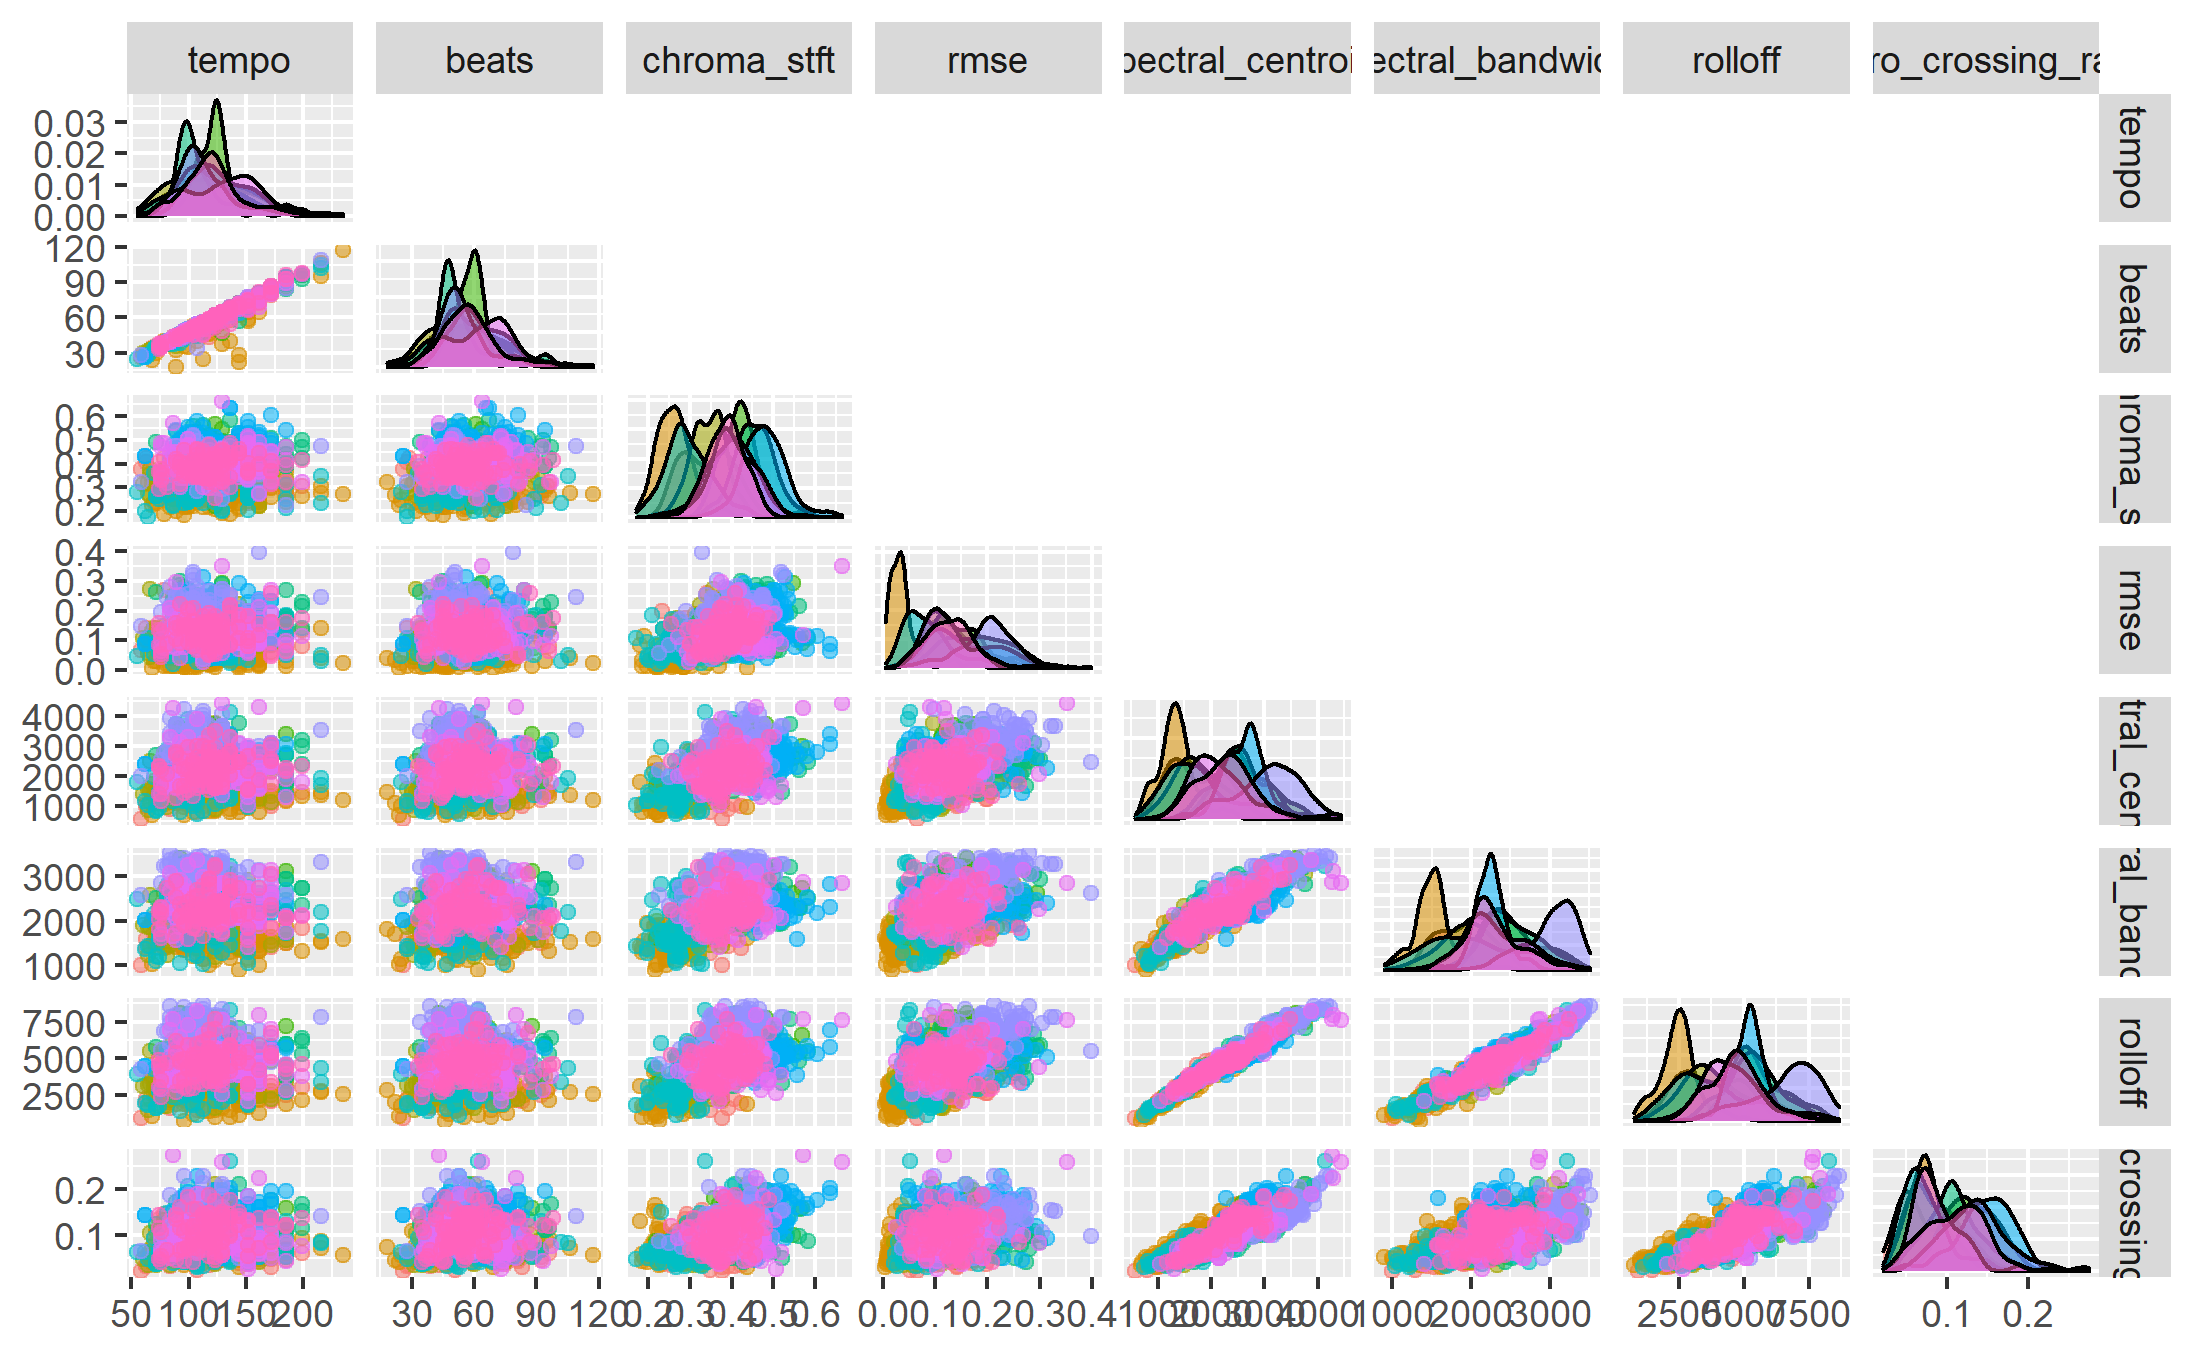
\includegraphics[width=0.9\textwidth]{ggpairs1.png}
    \end{center}
    \caption{Pars plot by ggplot}
\end{figure}
There is a high correlation between tempo and beats, and the tempo is about two times of beats. Moreover, spectral-centroid, spectral-bandwidth and rolloff are the results of spectral analysis, they must have correlation for each variables. 
\subsection{PCA (Principle Component Analysis)}
\begin{figure}[h]
\centering
    \begin{tabular}{c c}
        \textbf{\underline{PCA for features}} & \textbf{\underline{PCA for audios}} \\
        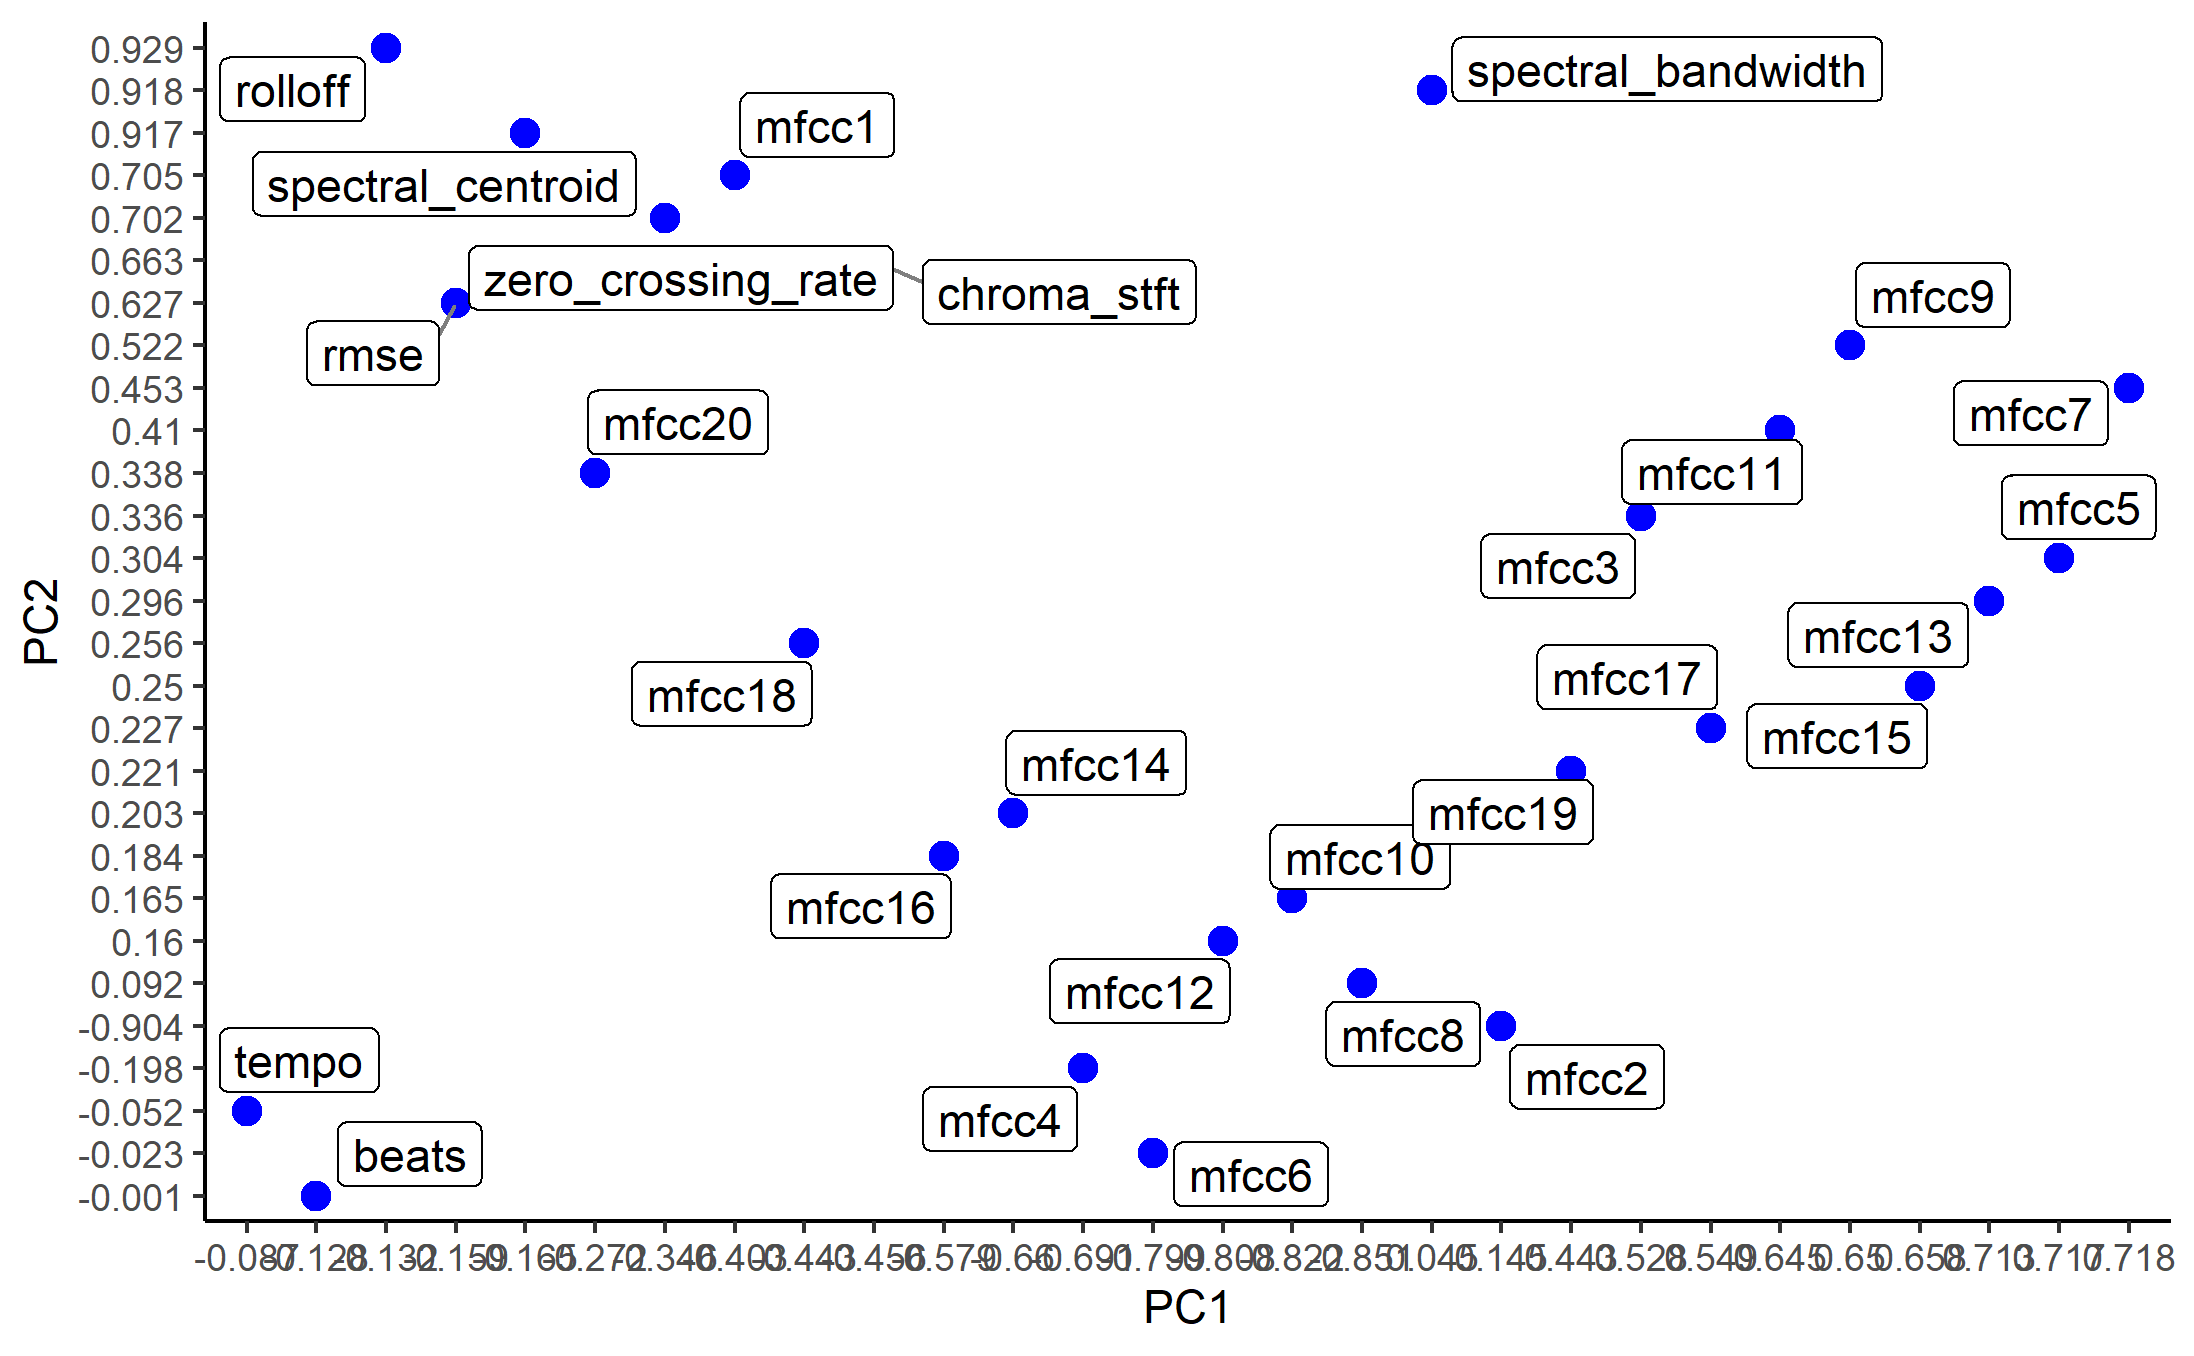
\includegraphics[width=0.5\textwidth]{pca_feat.png} & 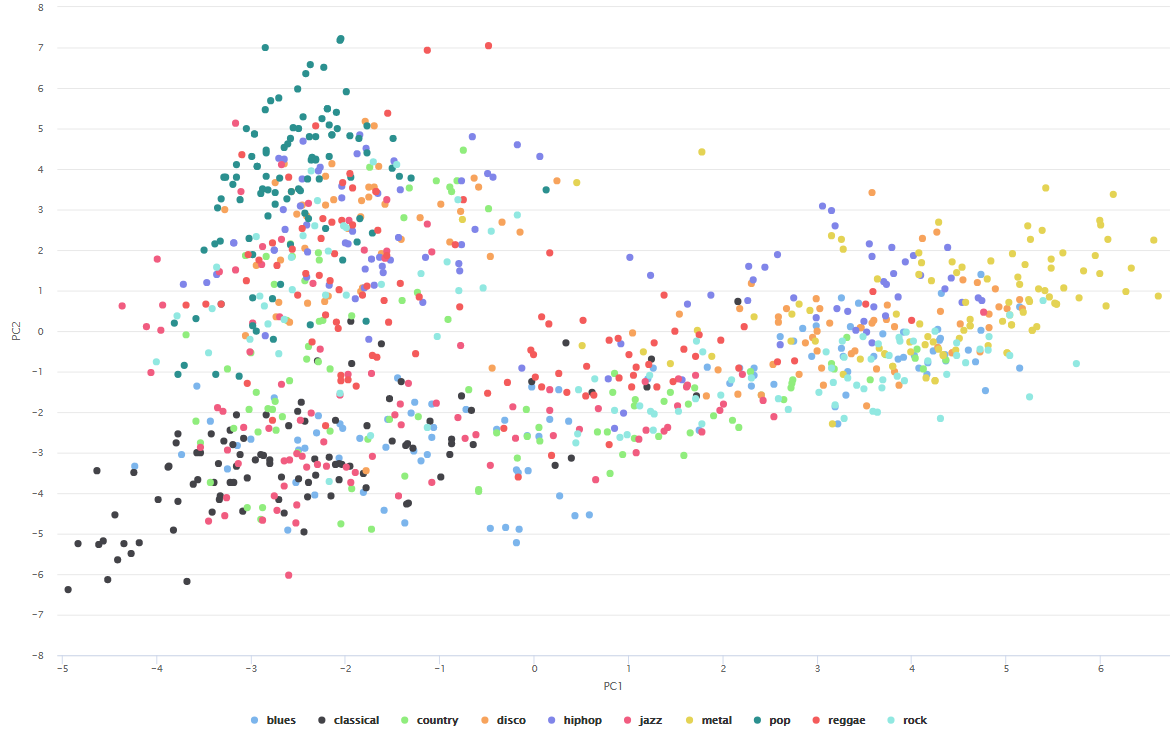
\includegraphics[width=0.5\textwidth]{pca.png}
    \end{tabular}
\caption{PCA}
\end{figure}

\section{Models}
\subsection{Training and Testing data}
For the balance in this data, taking $80\%$ as training data and $20\%$ as testing data from each genres, so training data contains 10 genres, each represented by 80 tracks. And so does testing data.
\subsection{Logistic Regression}
\begin{figure}[h]
    \begin{center}
        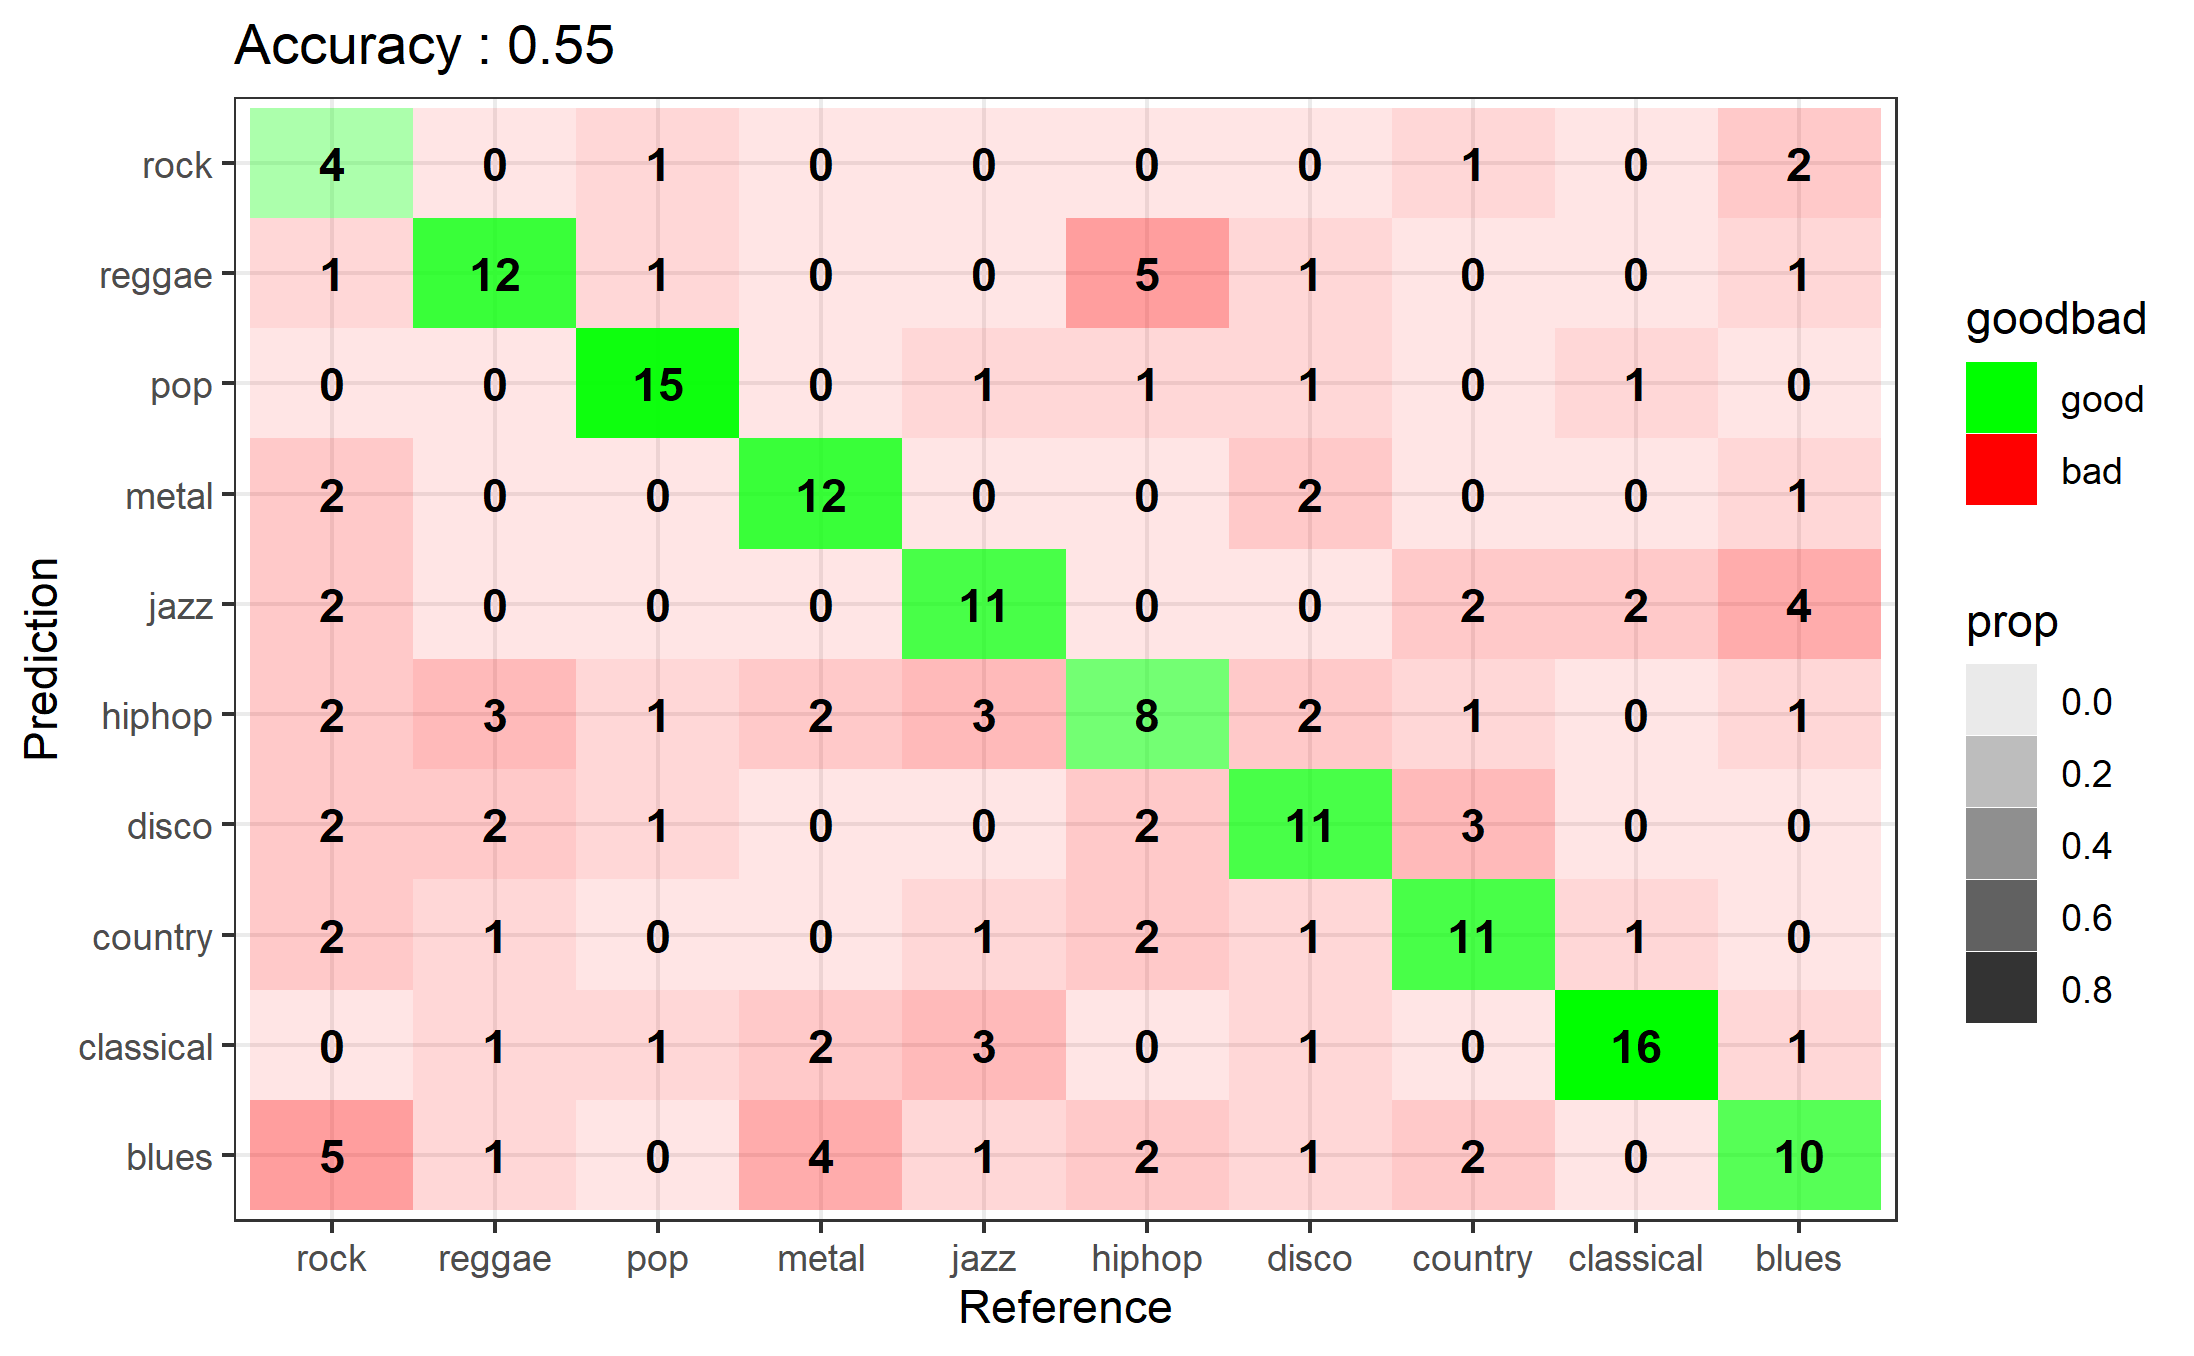
\includegraphics[width=0.7\textwidth]{confusionMatrix_logreg.png}
    \end{center}
    \caption{Confusion matrix: logistic regression}
\end{figure}
\newpage
\subsection{SVM (Support Vector Machine)}
\begin{figure}[h]
    \begin{center}
        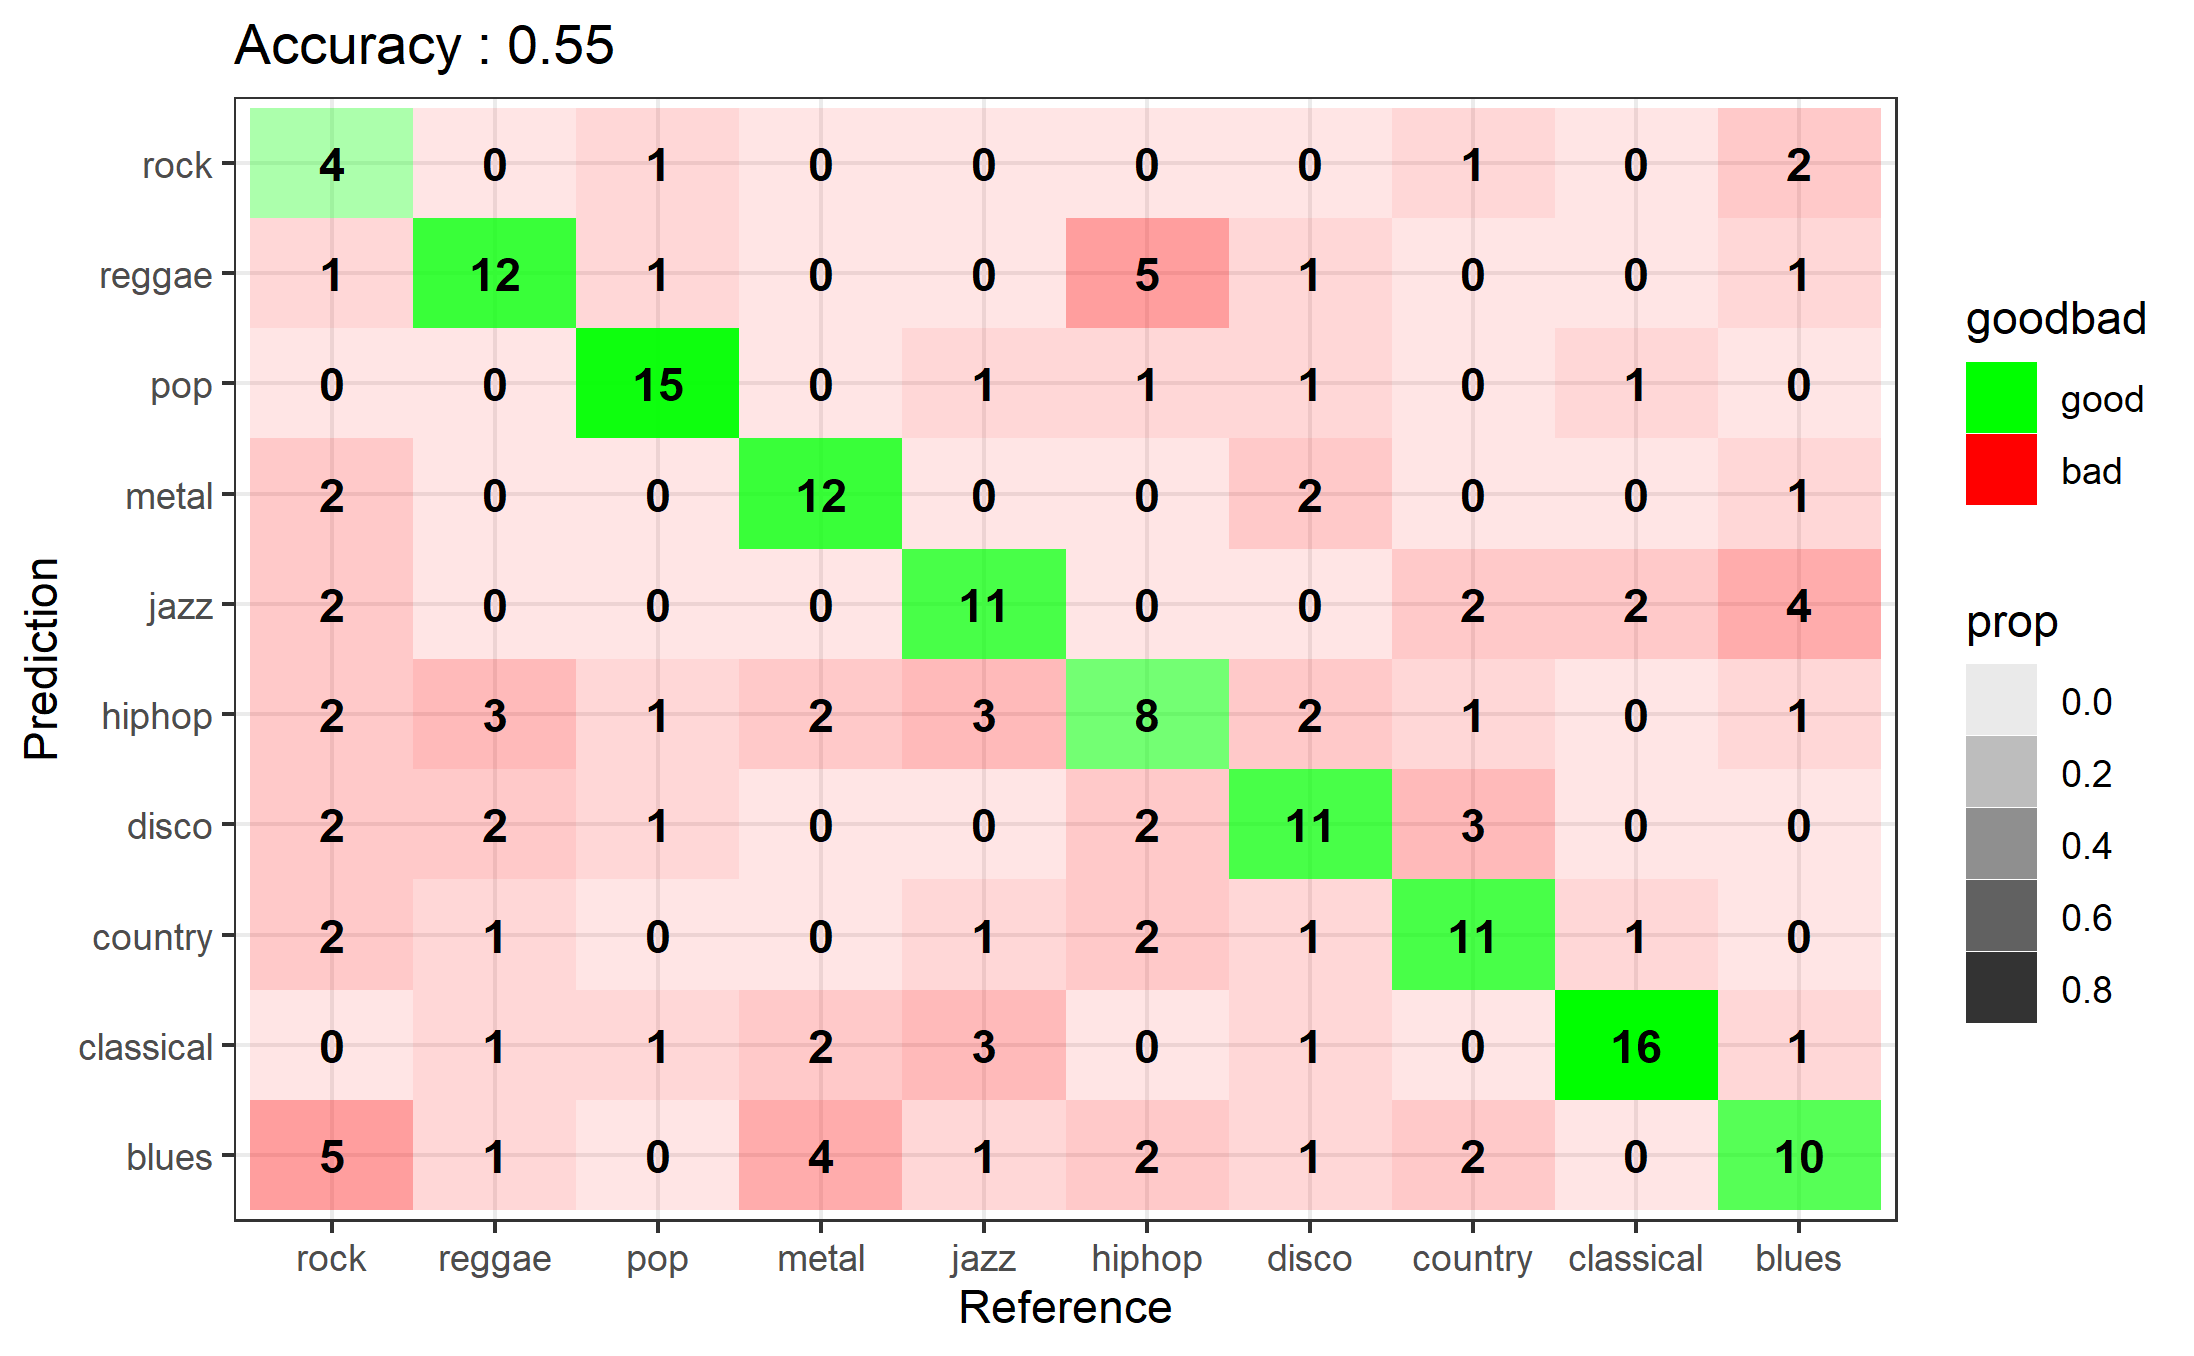
\includegraphics[width=0.7\textwidth]{confusionMatrix_logreg.png}
    \end{center}
    \caption{Confusion matrix: SVM}
\end{figure}
\subsection{SVM (one-hot encoding)}
Turning this 10 class prediction into a simple version, We do the one-hot encoding for the genres as the figure down below.
\begin{center}
    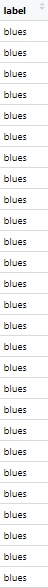
\includegraphics[width=0.043\textwidth]{y.jpg}$\Longrightarrow$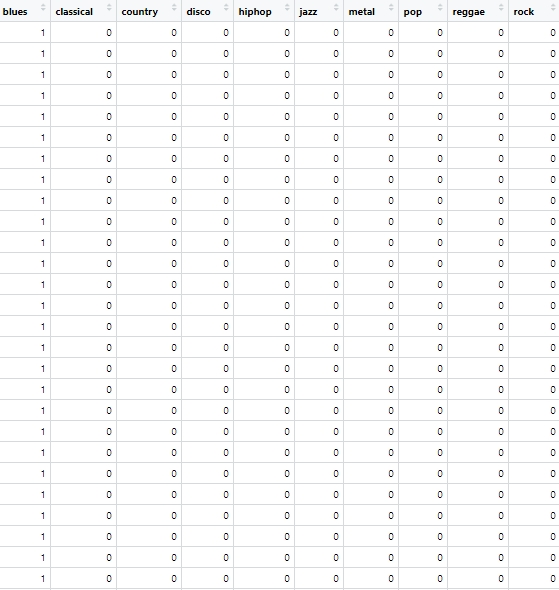
\includegraphics[width=0.5\textwidth]{y_matrix.jpg}
\end{center}
\newpage
\begin{figure}[h]
    \begin{center}
        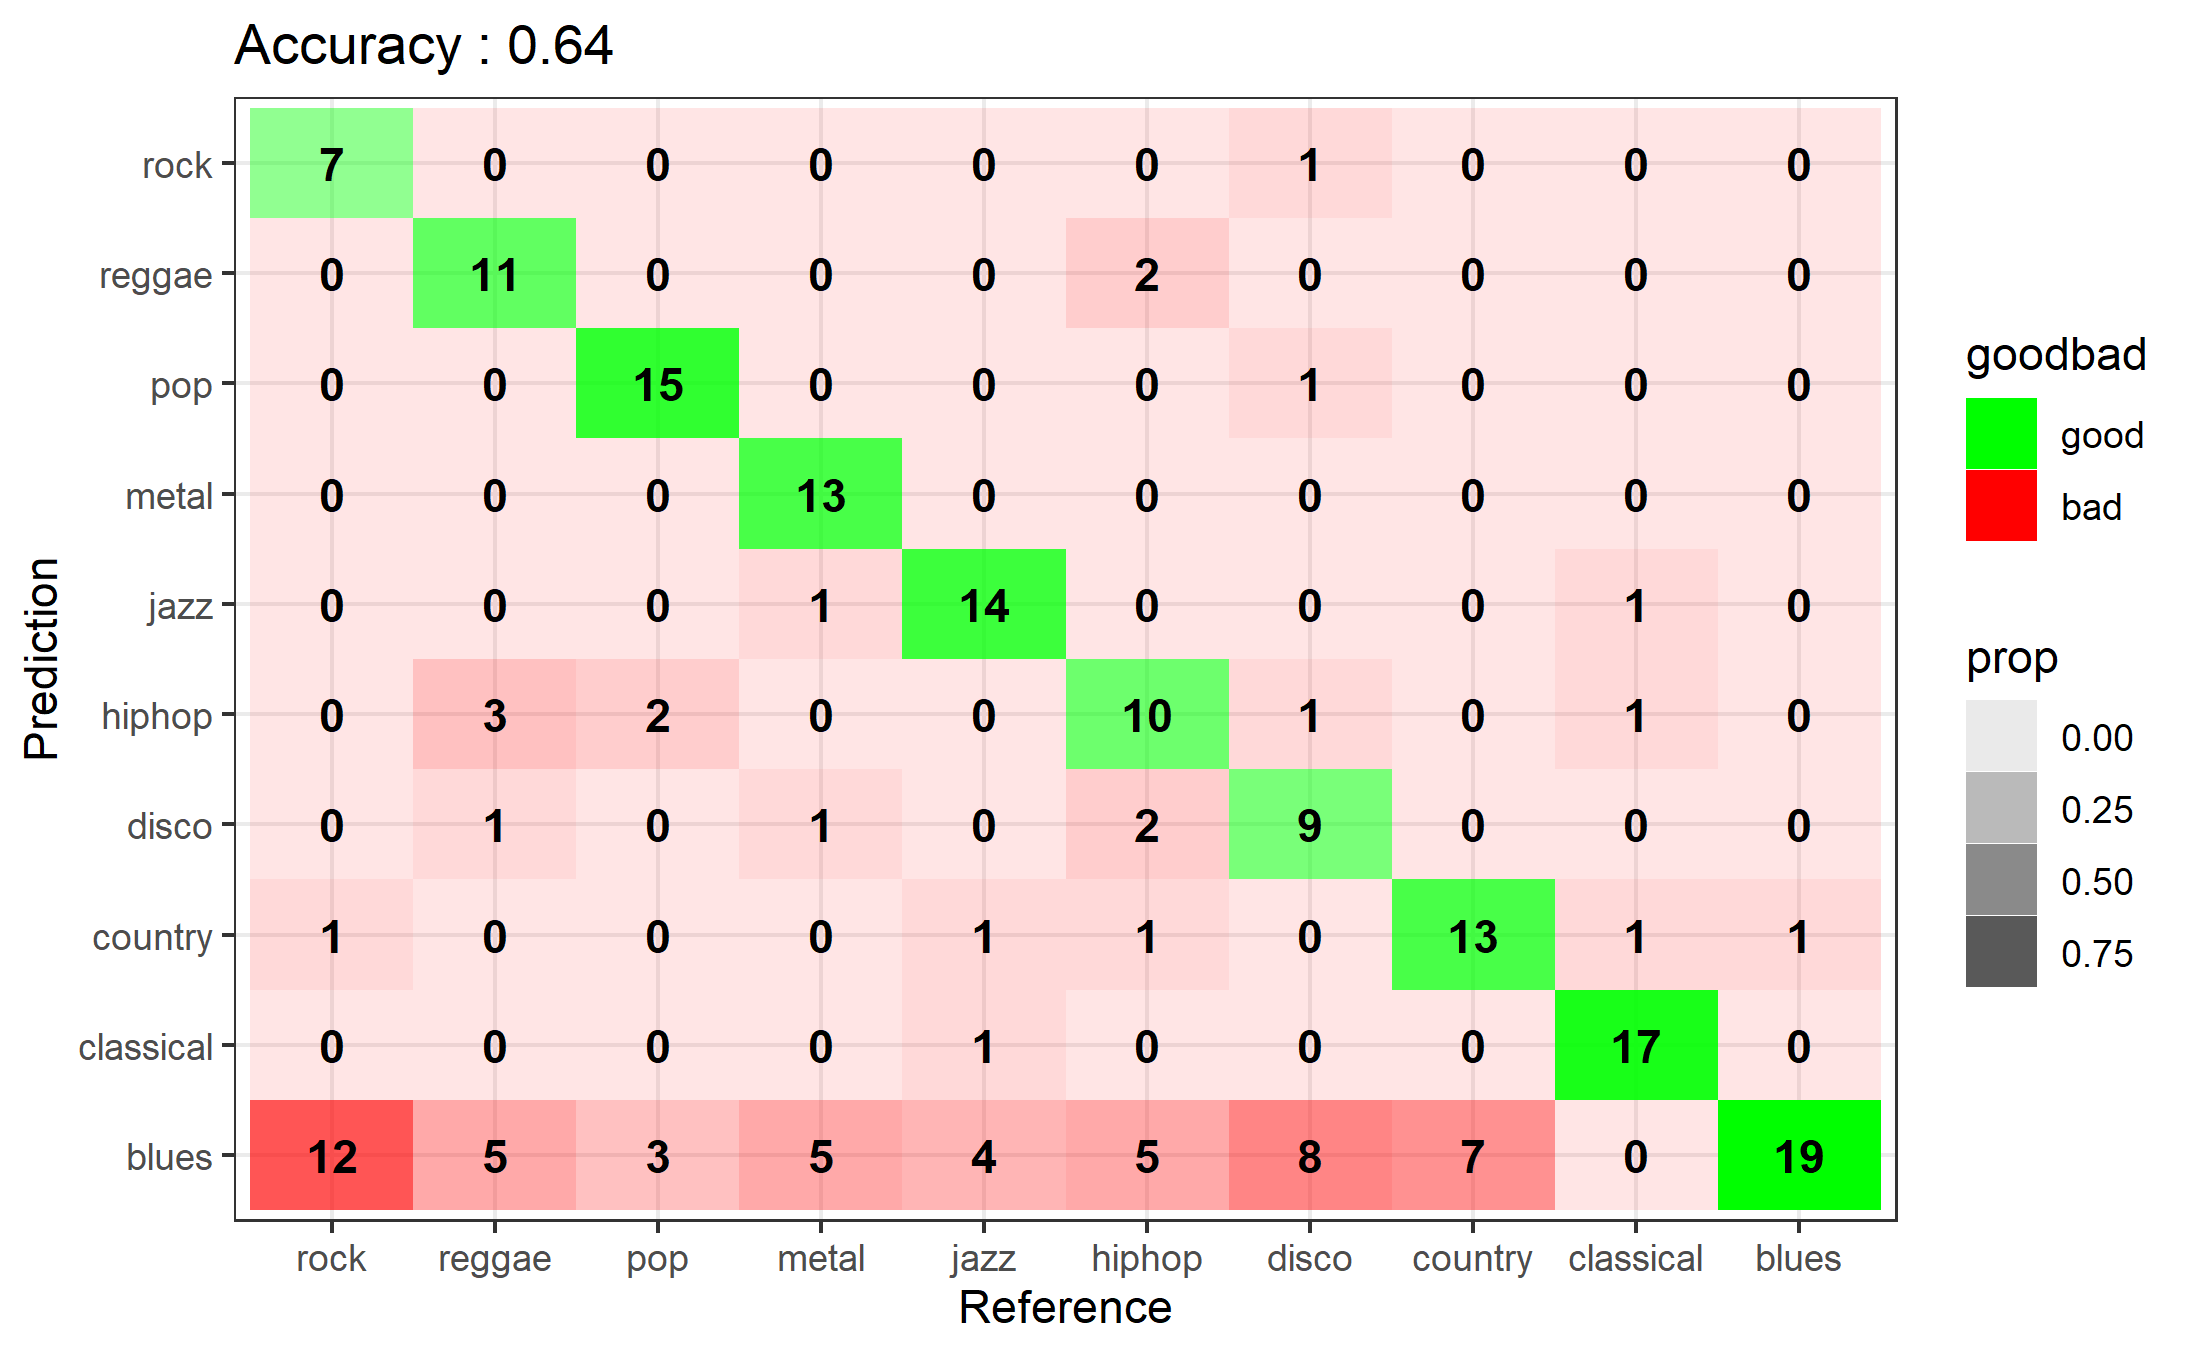
\includegraphics[width=0.7\textwidth]{confusionMatrix_ohencoding_std.png}
    \end{center}
    \caption{Confusion matrix: SVM (one-hot encoding)}
\end{figure}
\subsection{SVM (scaling)}
After reading the paper of tuning of SVM, scaling is very essential.
\begin{figure}[h]
    \begin{center}
        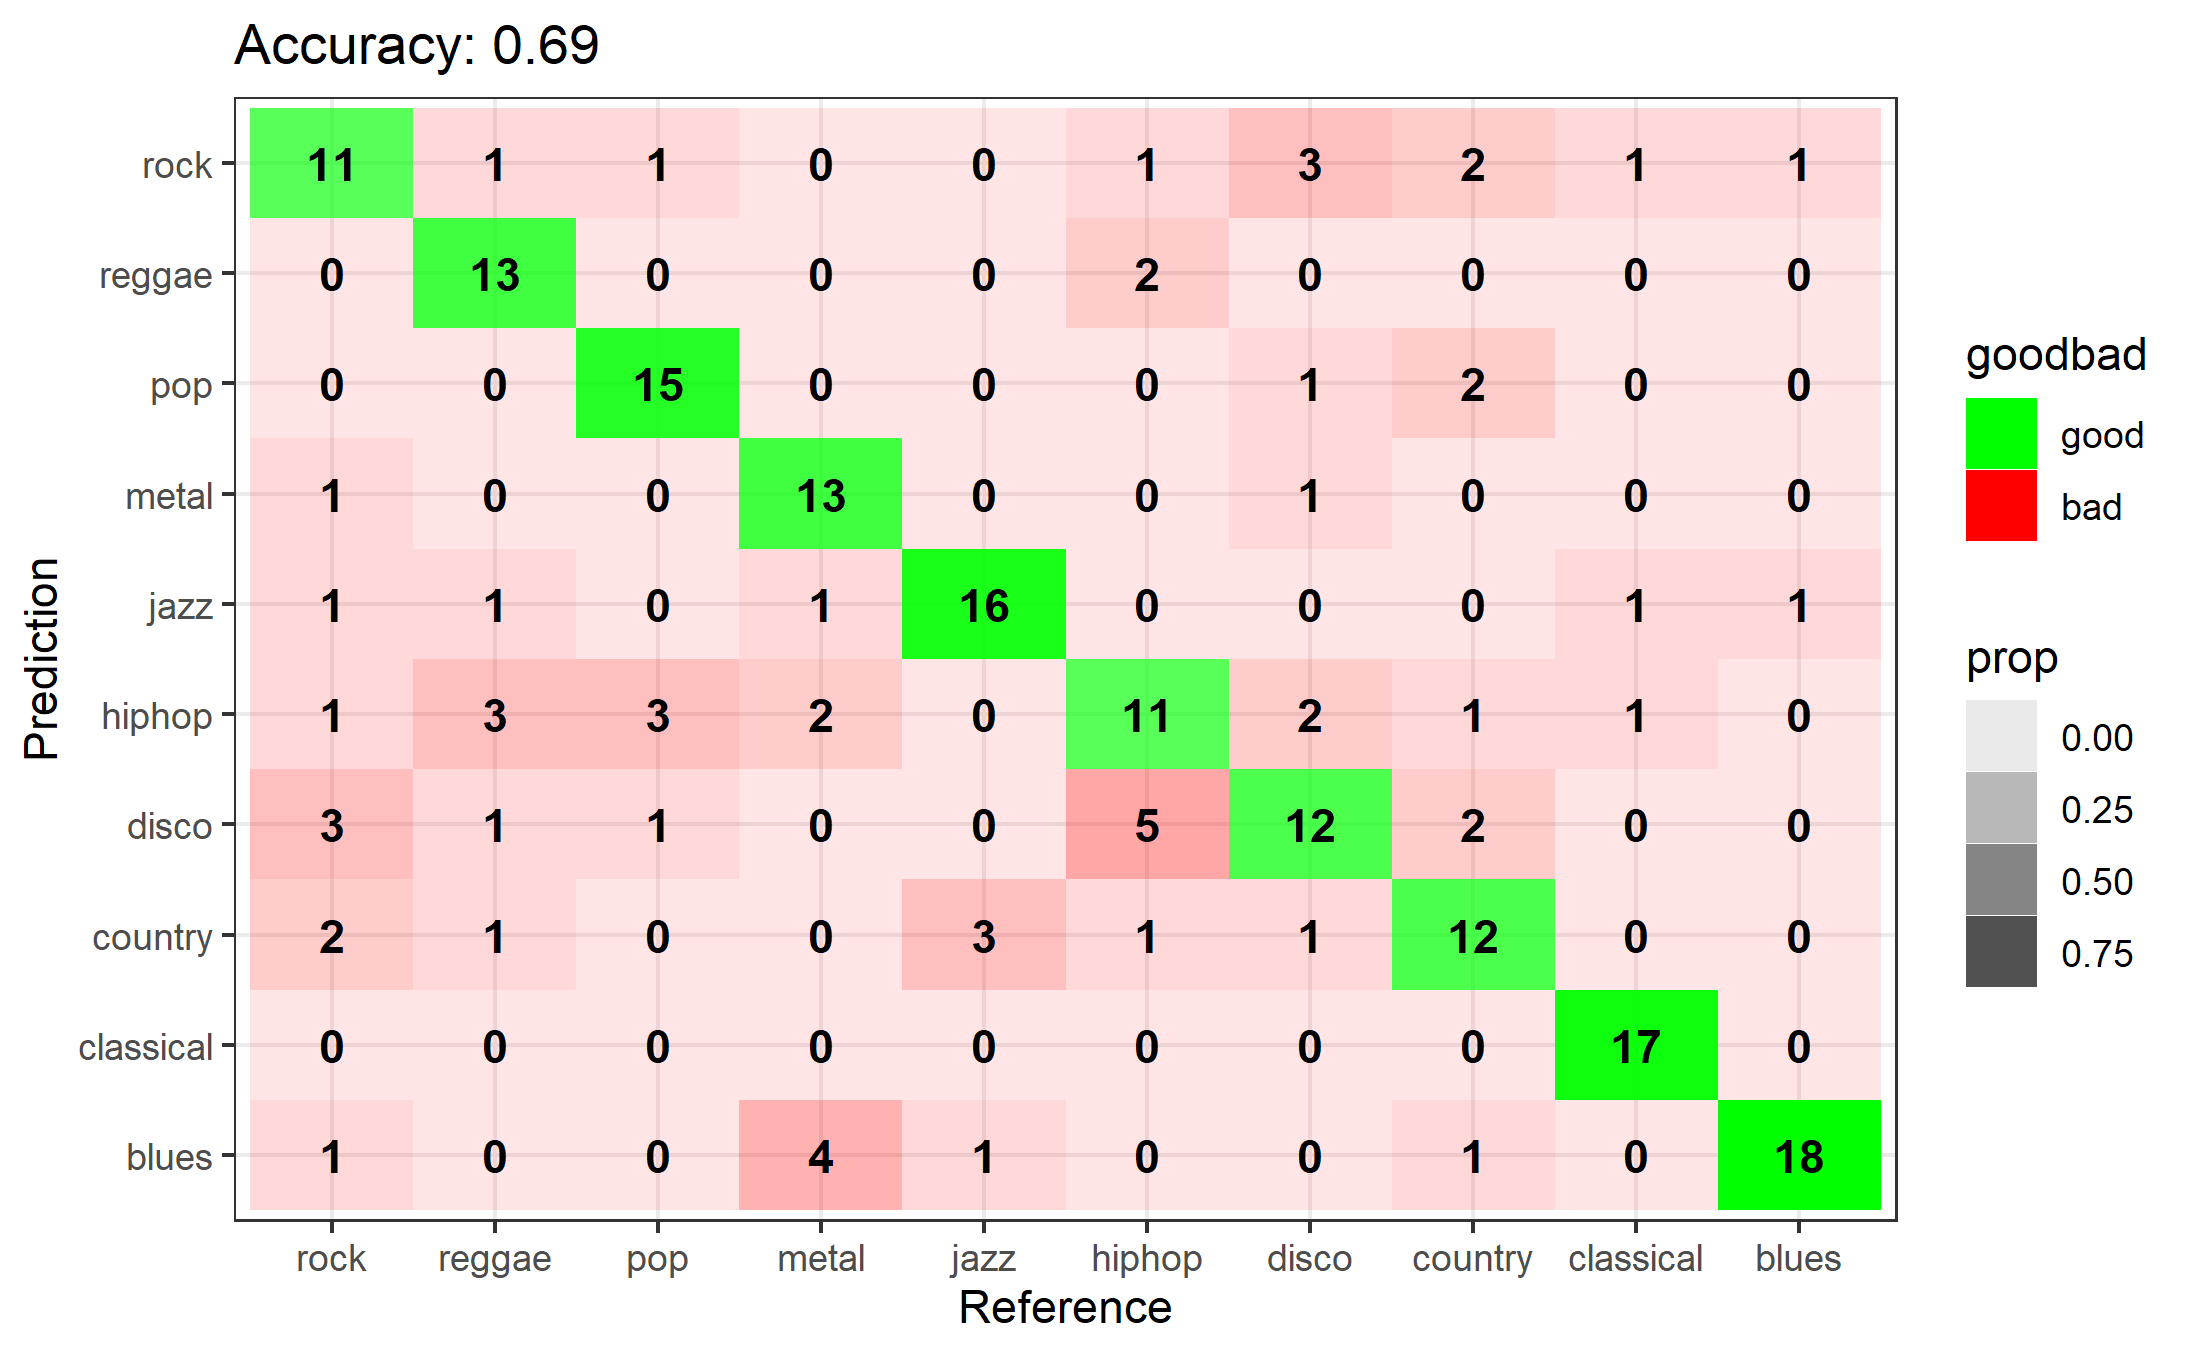
\includegraphics[width=0.7\textwidth]{confusionMatrix_svm_std.png}
    \end{center}
    \caption{Confusion matrix: SVM (scaling)}
\end{figure}
\newpage
\subsection{Random Forest}
\begin{figure}[h]
    \begin{center}
        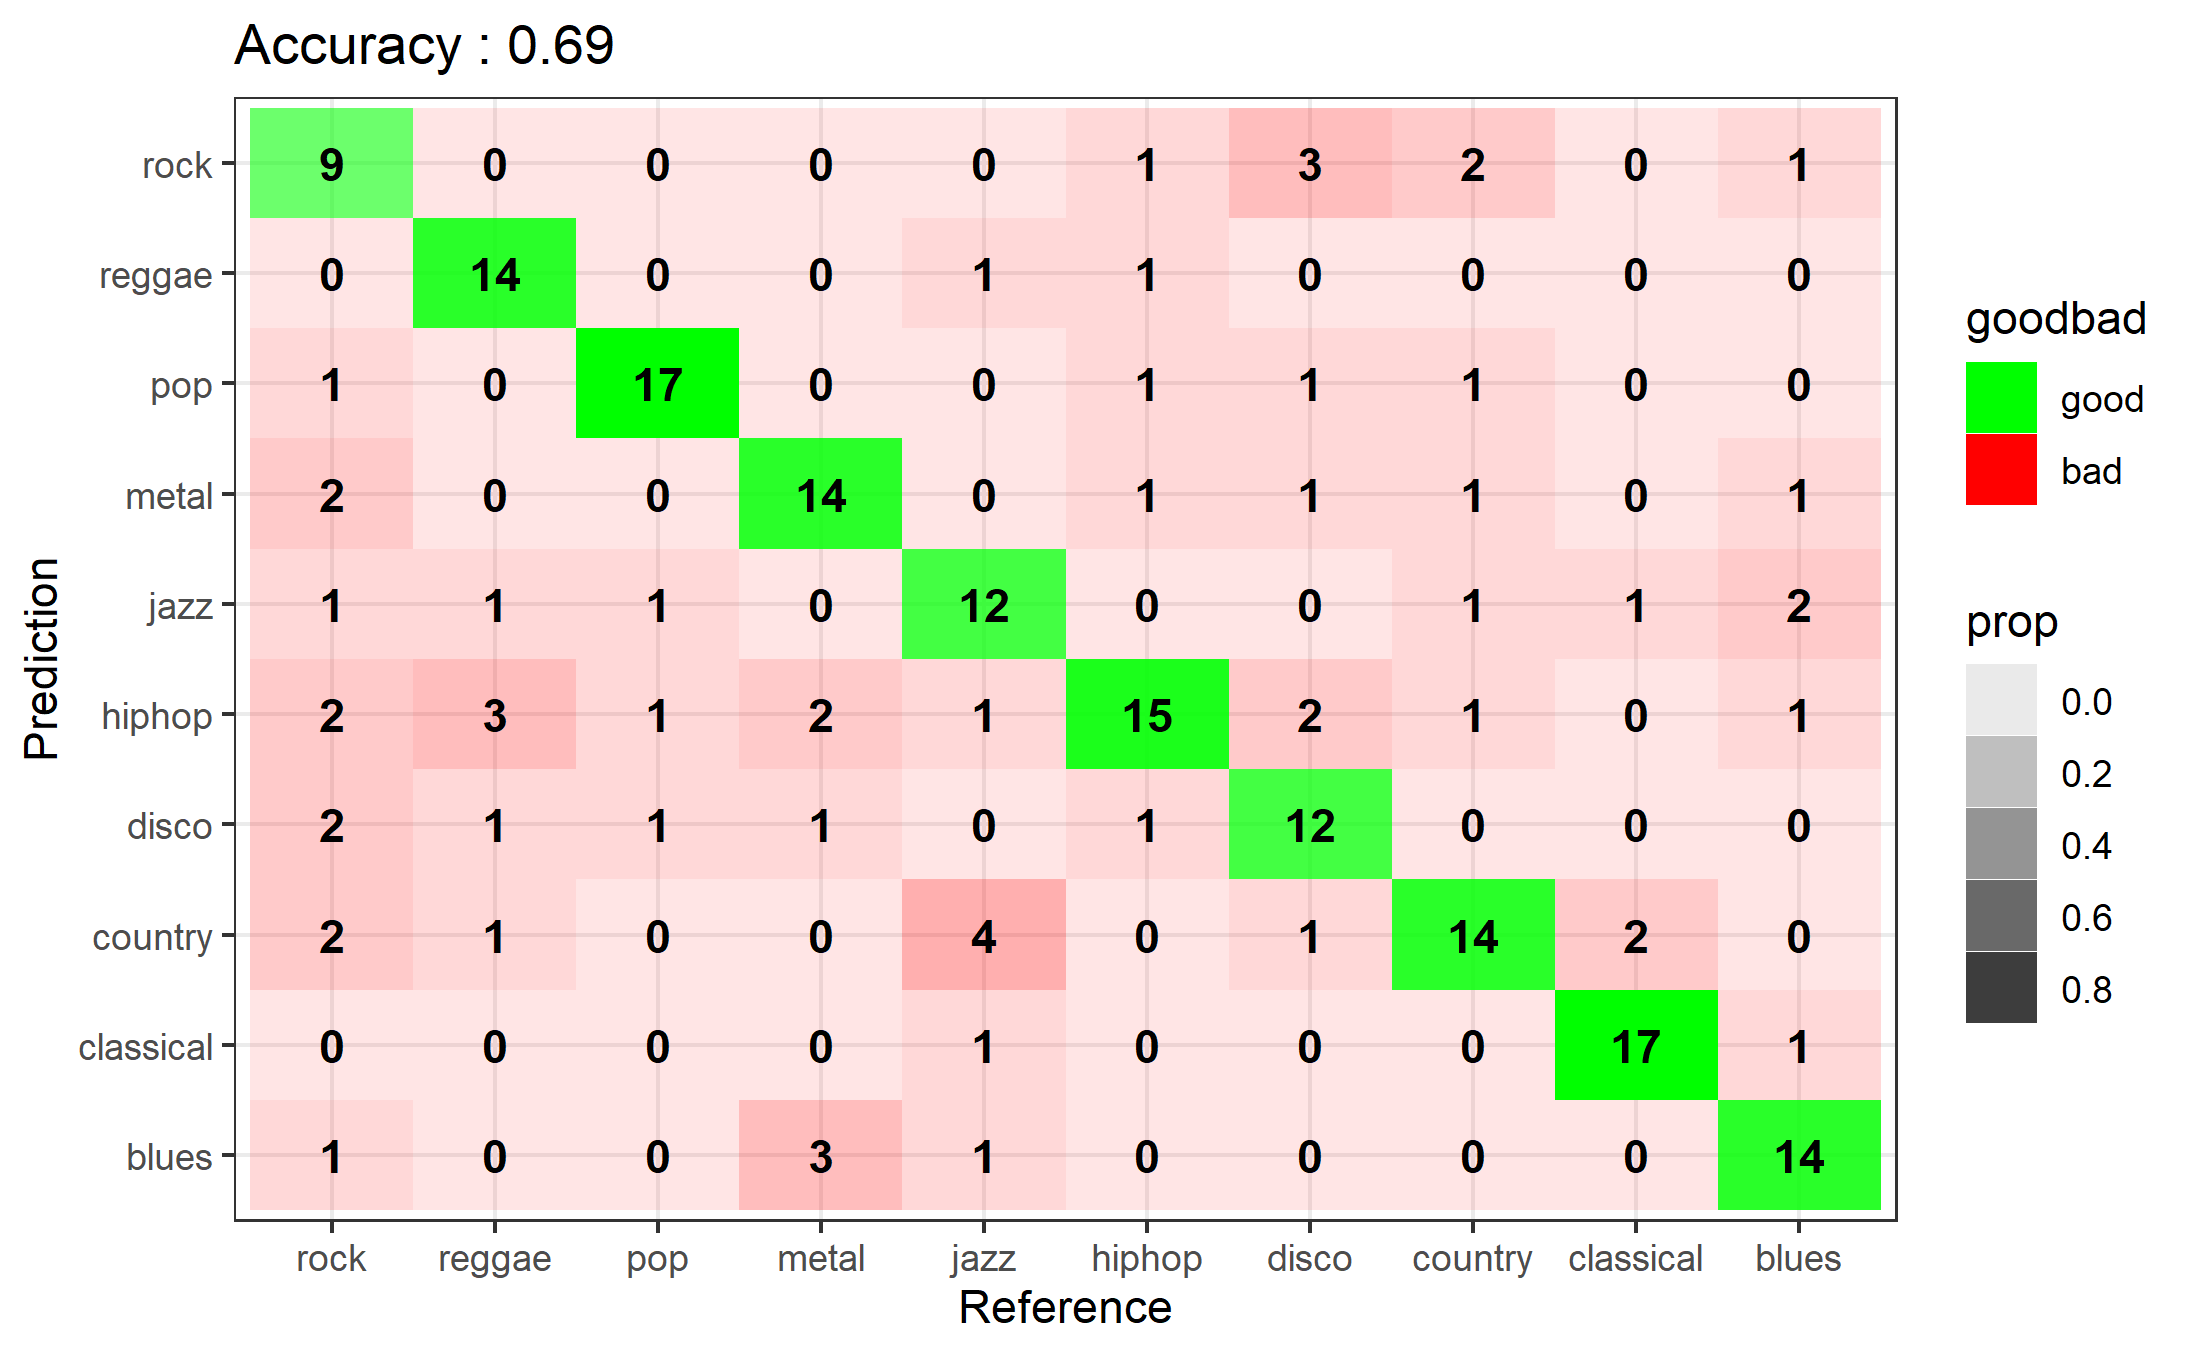
\includegraphics[width=0.7\textwidth]{confusionMatrix_randomforest.png}
    \end{center}
    \caption{Confusion matrix: Random forest}
\end{figure}
\subsection{Random Forest (scaling)}
\begin{figure}[h]
    \begin{center}
        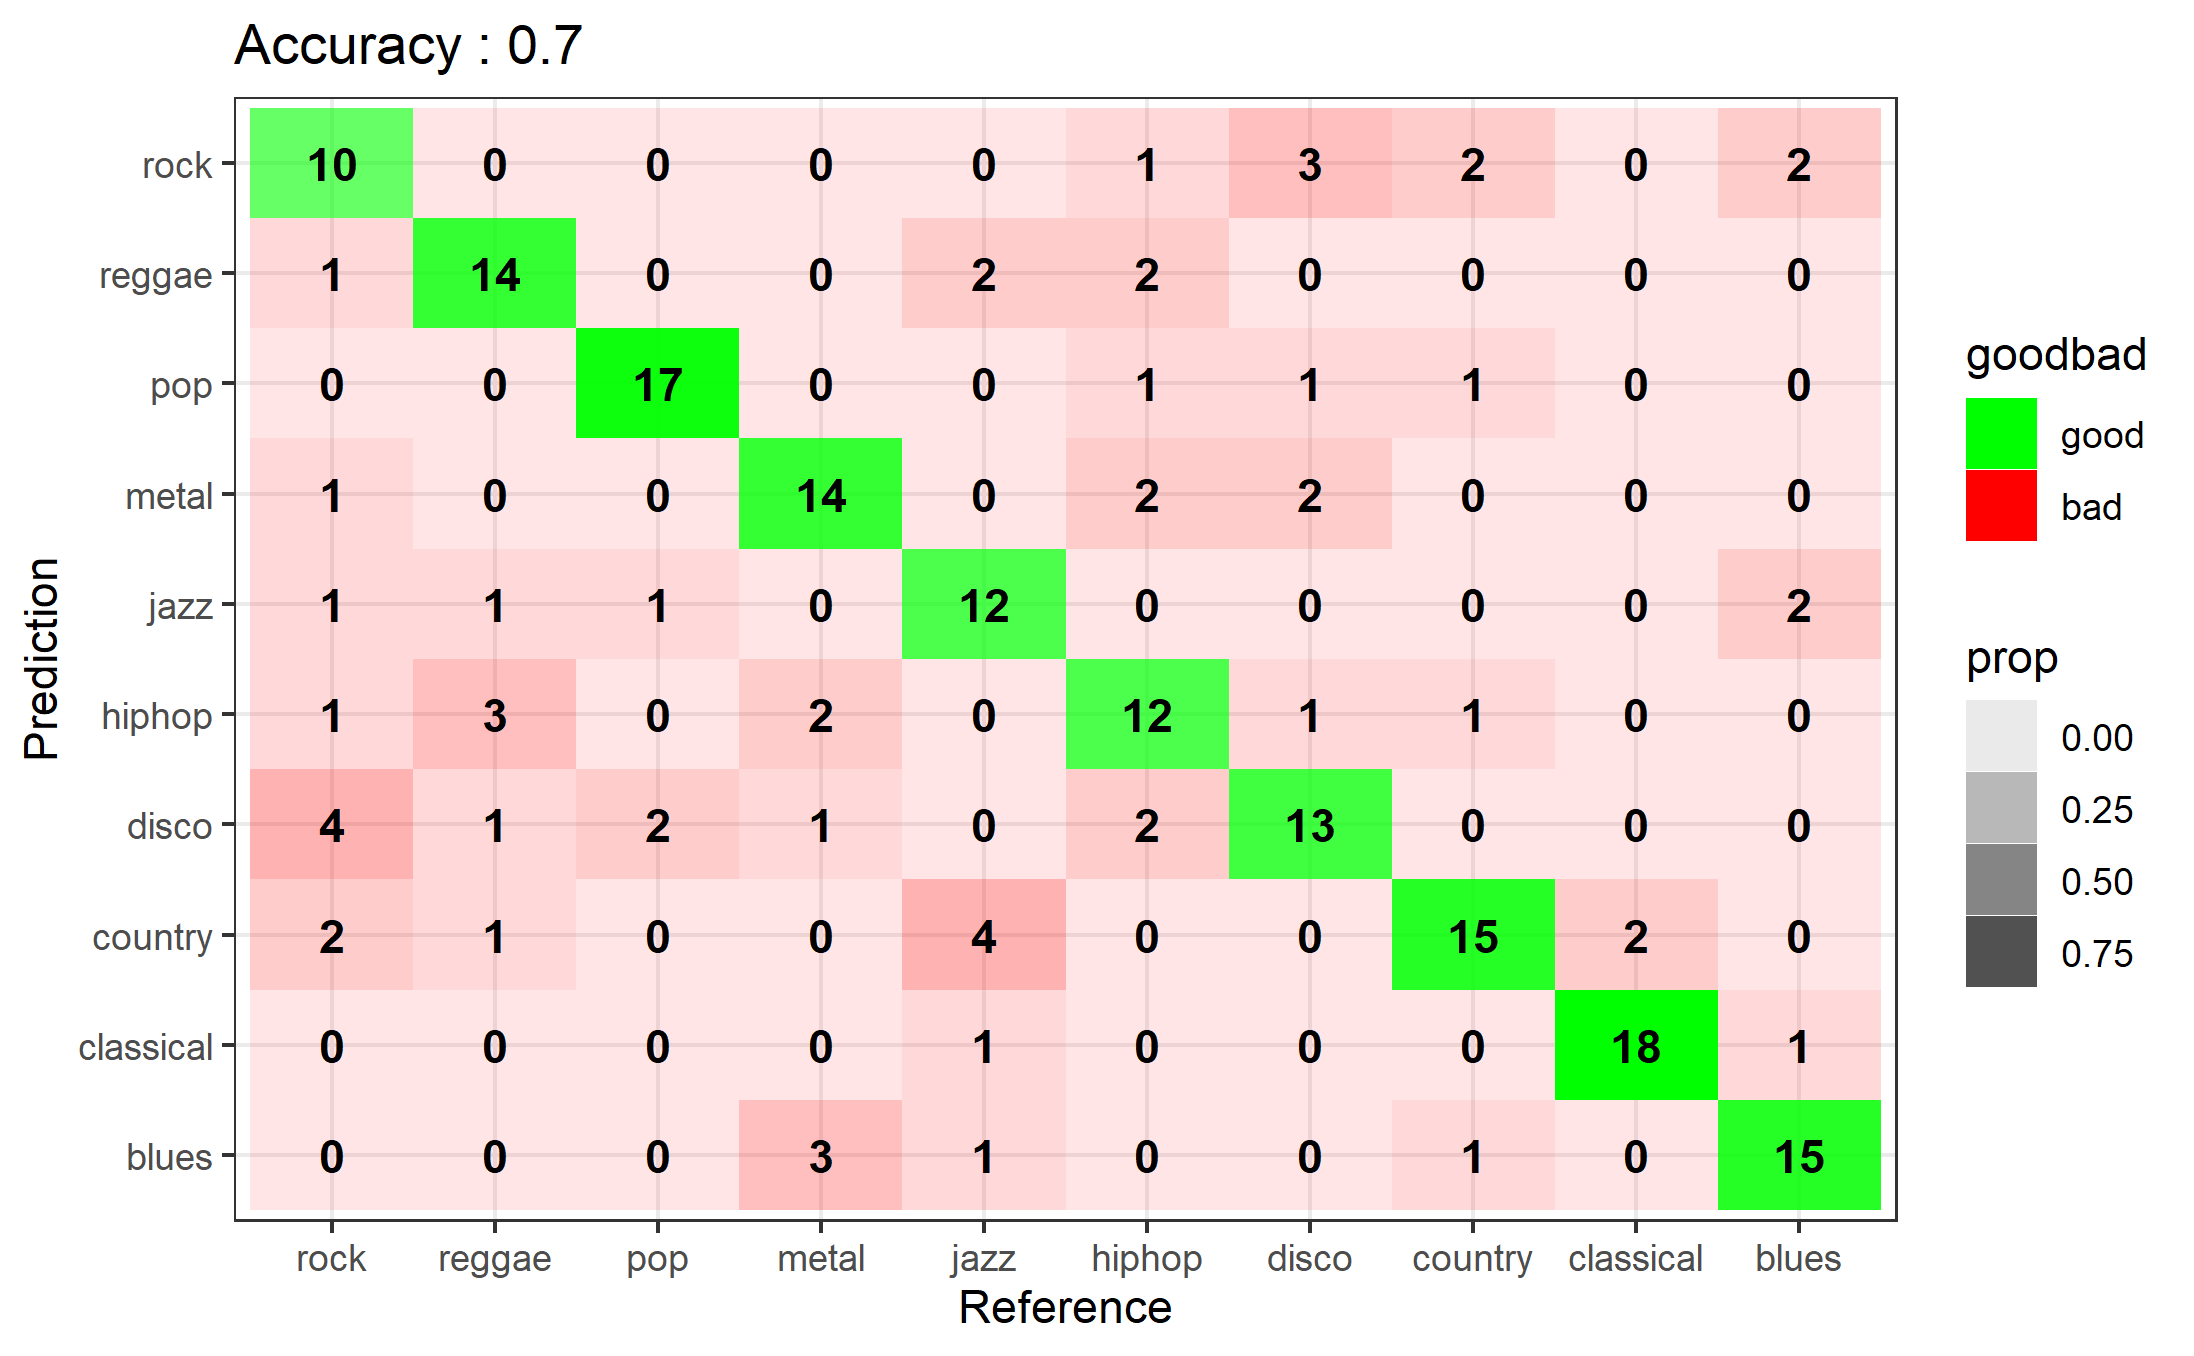
\includegraphics[width=0.7\textwidth]{confusionMatrix_randomforest_std.png}
    \end{center}
    \caption{Confusion matrix: Random forest (scaling)}
\end{figure}
\newpage
\section{Conclusions}
\begin{itemize}
  \item The music could be classified by 28 features extracted from signal transform and Fourier analysis.
  \item SVM and Random Forest are satisfactory classifier for this dataset.
\end{itemize}
\begin{center}
\begin{tabular}{ |c|c| } 
\hline
 model & accuracy \\ 
\hline
 logistic regression & 0.55 \\ 
 \hline\hline
 svm(one-hot encoding) & 0.64 \\ 
 \hline
 svm & 0.67 \\ 
 \hline
 svm(scaling) & 0.69 \\ 
 \hline\hline
 random forest & 0.69 \\ 
 \hline
 random forest(scaling) & 0.7 \\ 
 \hline
\end{tabular}
\end{center}

\newpage

\addcontentsline{toc}{section}{References}
\section*{References}
\begin{itemize}
  \item Trevor Hastie, Robert Tibshirani, Jerome Friedman, The Elements of Statistical Learning: Data Mining, Inference and Prediction, 2nd Edition, Springer, New York, 2009.
  \item Wolfgang Karl Härdle, Léopold Simar,  Applied Multivariate Statistical Analysis, 4th Edition, Springer, New York, 2015.
  \item Chih-Wei Hsu, Chih-Chung Chang, Chih-Jen Lin, A Practical Guide to Support Vector Classification. \url{https://www.csie.ntu.edu.tw/~cjlin/papers/guide/guide.pdf}, 2016 (accessed April 12 2022).
  \item Meinard Muller, Stefan Balke, Short-Time Fourier Transform and Chroma Features. \url{https://www.audiolabs-erlangen.de/content/05-fau/professor/00-mueller/02-teaching/2020s_apl/1_stft/stft_and_chroma_features.html}, 2015 (accessed June 2 2022).
  \item Kaggle: Music Features, \url{https://www.kaggle.com/datasets/insiyeah/musicfeatures}, (accessed April 2 2022)
  \item Python package Librosa, \url{https://librosa.org/doc/latest/index.html}, 2013 (accessed June 2 2022)
  \item What's the Difference Between Tempo and Rhythm?, \url{https://www.britannica.com/story/whats-the-difference-between-tempo-and-rhythm}, (accessed June 2 2022)
\end{itemize}

\end{document}